\section{Aktører}

% Kontekst diagram
\begin{figure}[H] \centering
    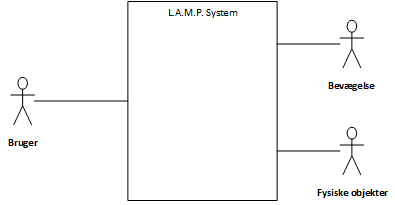
\includegraphics[width=\textwidth]{0_Filer/Figuer/AktoerKontekstLAMP.png}
    \caption{Kontekst diagram}
    \label{fig:kontekstdiagram}
\end{figure}

% Bruger
\begin{table}[H] \centering
\subsection{Bruger}
\begin{tabular}{|p{4cm}|p{8cm}|}
	\hline
	    \textbf{Alternativ reference}   & Ingen \\ \hline
	    \textbf{Type}                   & Primær \\ \hline
		\textbf{Beskrivelse}            & Brugeren interagerer med systemet via GUI. \\ \hline
	\end{tabular}
\end{table}

% Bevægelse
\begin{table}[H] \centering
\subsection{Bevægelse}
    \begin{tabular}{|p{4cm}|p{8cm}|}
	\hline
	    \textbf{Alternativ reference}   & Ingen \\ \hline
	    \textbf{Type}                   & Sekundær \\ \hline
		\textbf{Beskrivelse}            & Bevægelse i rummet vil aktivere bevægelsessensoren som vil tænde lys. \\ \hline
	\end{tabular}
\end{table}

% Fysiske Objekter
\begin{table}[H] \centering
\subsection{Fysiske Objekter}
\begin{tabular}{|p{4cm}|p{8cm}|}
	\hline
	    \textbf{Alternativ reference}   & Ingen \\ \hline
	    \textbf{Type}                   & Sekundær \\ \hline
		\textbf{Beskrivelse}            & Fysiske Objekter vil, hvis i en given afstand under lampen, stoppe nedadgående bevægelse. \\ \hline
	\end{tabular}
\end{table}